\chapter{Results and Discussion}

Here we examine both the performance and visual quality of our global illumination algorithm. The primary means of evaluating performance is based on GPU memory usage and frame time. The times of each contributing render pass are also recorded. Evaluating visual quality is based largely on whether the lighting appears smooth and believable with a minimal amount of noise and artifacts.

We also discuss the application of voxel warping and how it compares with other global illumination methods. Unfortunately, direct performance and visual quality comparisons are difficult to objectively measure as there are many contributing factors---mesh complexity and optimizations, texture resolution and format, shading model, graphics API, hardware, GPU driver version, etc.---that affect the final comparison, in addition to the exact implementation details. Nevertheless, we provide motivations and tradeoffs between our method and others and their potential impact on performance and quality.

\section{Test Setup}
% TODO verify driver, kernel, resolution when getting final results
All results are obtained from a system with an i5-2400 CPU, 8GB of DDR3 RAM, and an NVIDIA GeForce GTX 970 GPU. The system is running Arch Linux kernel 4.16.8-1 and uses the proprietary NVIDIA graphics driver version 396.24. The application uses an OpenGL 4.5 context and the scene is rendered with a window resolution of 1920x1080.

% TODO give #vertices, texture resolutions and sizes?
The model used in the test scenes is the Crytek Sponza scene. The textures from the original Sponza scene are replaced with ones necessary for PBR (materials are defined by a diffuse color, roughness, metallic coefficient, normal, and optionally an alpha texture). Mipmaps for the original textures were also precomputed and stored along with the full size 1024x1024 textures as DDS (Microsoft DirectDraw Surface) files using the compressed DXT5 format for faster scene loading.

To measure performance timings for each render pass we make use of OpenGL timer queries using the \verb#GL_TIME_ELAPSED# query type. The results of the query object are double buffered to ensure introducing the timer query does not affect the total render time.

Unless otherwise mentioned, voxel resolutions are 256x256x256 with 6 mipmap levels.

\section{Analysis}
In the following sections we evaluate various aspects of our work. First, we discuss the global illumination algorithm as a whole. Second, we compare the rasterization-based and tesselation-based voxelization algorithms. Lastly, we provide the results of our voxel warping and some insights on future improvements.

\subsection{Global Illumination}
Table~\ref{tbl:renderpasstiming} shows timing results from the complete global illumination algorithm. We test the algorithm with different screen resolutions and voxel grid resolutions. Recall that a minimum goal for real-time is 30 frames per second and a target is 60 frames per second, which correspond to individual frame times of 33.3ms and 16.7ms, respectively. We see that the total frame time always meets the goal of 60 frames per second.

The data shows that shadowmap creation and radiance injection was independent of screen resolution and voxel resolution\footnote{As expected, since the main factor for both of these render passes is the size of the shadowmap, which remained constant at 4096x4096.}. The voxelization and radiance filtering steps both only depended on voxel grid resolution. The depth prepass also only varied with respect to screen resolution. The final shading predictably depended on both voxel grid resolution and screen resolution. However, larger voxel grid resolutions did not affect the final shading times by much at a given screen resolution, with approximately a 1.5ms difference between using a voxel resolution of 64 versus 256.

\begin{table}[H]
\centering
\begin{tabular}{l ccc ccc ccc}
\toprule
Render Pass & \multicolumn{9}{c}{Render Pass Time (ms)} \\
& \multicolumn{3}{c}{1280x720} & \multicolumn{3}{c}{1600x900} & \multicolumn{3}{c}{1920x1080} \\
& 64 & 128 & 256 & 64 & 128 & 256 & 64 & 128 & 256 \\
\midrule
Voxelize           & 0.90 & 1.13 & 2.40  & 0.70 & 1.12 & 2.39  & 0.72 & 1.15 & 2.41\\
Shadowmap          & 0.69 & 0.69 & 0.69  & 0.69 & 0.69 & 0.69  & 0.68 & 0.68 & 0.69\\
Radiance Injection & 0.92 & 0.92 & 0.93  & 0.92 & 0.92 & 0.93  & 0.92 & 0.92 & 0.93\\
Radiance Filtering & 0.04 & 0.10 & 0.55  & 0.05 & 0.10 & 0.56  & 0.04 & 0.10 & 0.55\\
Depth Prepass      & 0.20 & 0.20 & 0.20  & 0.25 & 0.26 & 0.25  & 0.31 & 0.31 & 0.36\\
Final Shading      & 3.89 & 4.81 & 5.32  & 5.98 & 6.42 & 7.10  & 8.23 & 9.40 & 9.75\\
\midrule
Total              & 7.02 & 8.21 & 11.12  & 9.46 & 10.15 & 13.43  & 11.23 & 12.83 & 16.31\\
\bottomrule
\end{tabular}
\caption{Times measured for each render pass for various screen resolutions and voxel grid resolutions. The total timer also accounts for any other operations performed within each frame (i.e.\ the sum of the render pass times is not necessarily the complete time for an entire frame). Voxelization is done using the tesselation-based approach.}
\label{tbl:renderpasstiming}
\end{table}

\subsection{Tesselated Voxelization}
In terms of both performance and visual quality both voxelization methods are very similar. Voxelization times for each method are shown in Table~\ref{tbl:voxelizationtiming}, where we see the tesselation-based voxelization is slightly slower than the rasterization-based approach\footnote{However both implementations were not heavily optimized.}. Figure~\ref{fig:results_voxelization} compares the final rendered scene with both voxelization methods. The differences are minor.

Ultimately, both voxelization methods are sufficient for real-time global illumination. The (unoptimized) tesselation-based approach is slightly easier to implement and debug\footnote{Since the voxels are written in the tesselation evaluation stage, it is simple to add a geometry shader that takes the vertices and expands them into cubes, which are then rasterized and shaded with the vertex color (the same color inserted into the voxel texture).} but is slower than the rasterization-based approach.

\begin{figure}[h!]
\centering
    \begin{subfigure}[t]{0.4\textwidth}
        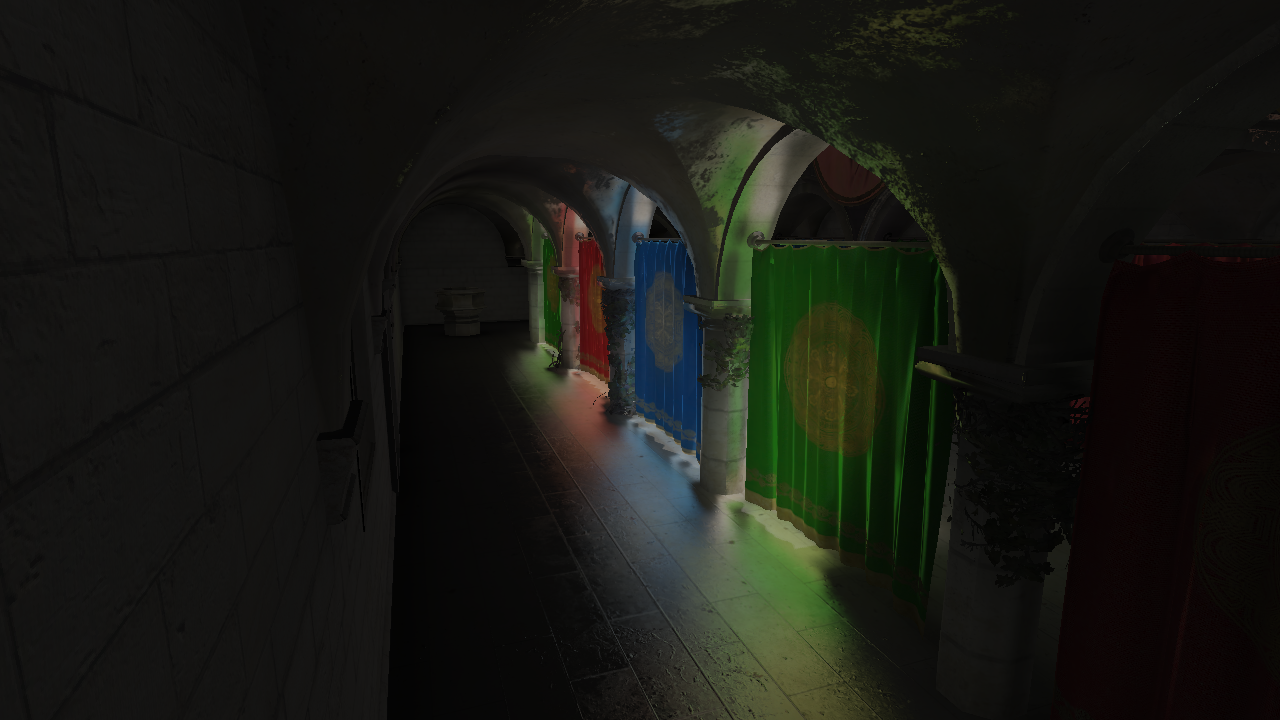
\includegraphics[width=\textwidth]{results_voxelraster.png}
        \caption{Rasterized voxels}
    \end{subfigure}
    ~
    \begin{subfigure}[t]{0.4\textwidth}
        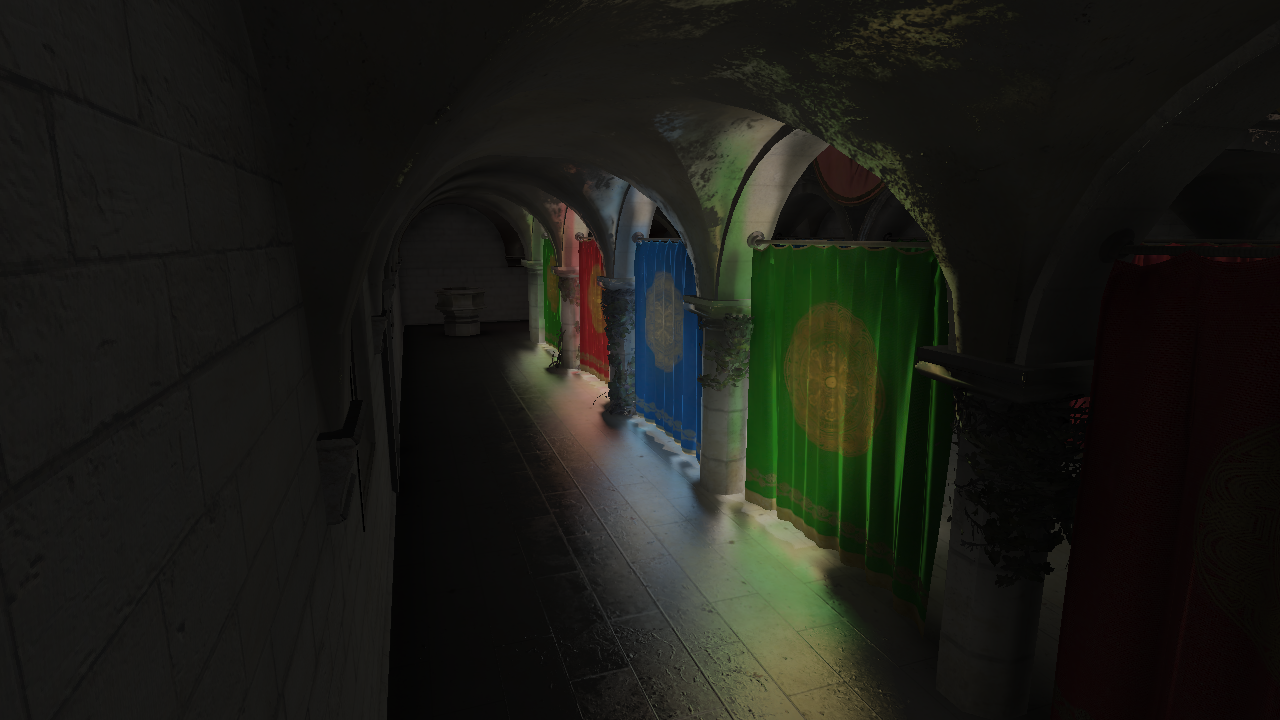
\includegraphics[width=\textwidth]{results_voxeltess.png}
        \caption{Tesselated voxels}
    \end{subfigure}
    \caption{The final rendered image for both voxelization methods have negligable visual differences.}
    \label{fig:results_voxelization}
\end{figure}

\begin{table}[H]
\centering
\begin{tabular}{lcc}
\toprule
\multirow{2}{*}{Voxel Grid Size} & \multicolumn{2}{c}{Voxelization Time (ms)} \\
& Rasterization-Based & Tesselation-Based \\
\midrule
64x64x64        & 0.53 & 0.70\\
128x128x128     & 0.85 & 1.12\\
256x256x256     & 1.91 & 2.35\\
\bottomrule
\end{tabular}
\caption{Time spent voxelizing the scene with varying voxel grid resolutions. For the rasterization-based approach the MSAA method of conservative rasterization is used.}
\label{tbl:voxelizationtiming}
\end{table}

\subsection{Integration of Voxel Cone Tracing into Existing Engines}
Voxel cone tracing is an attractive method for adding full global illumination to existing engines. The necessary information needed for the algorithm should already be available in most engines. A voxelized representation of the scene can be generated from any arbitrary triangle mesh using either of the voxelization methods presented. Other methods for voxelization could also be used if, for example, some geometry is generated procedurally. For radiance injection the only external inputs required are shadowmaps (or RSMs) for any lights that will contribute to the indirect lighting. Finally, the cone tracing needs surface normals and a TBN matrix (to transform the cone directions to world space), which will already be available for any engine which supports normal mapping.

\subsection{Voxel Warping}

% atomicMax vs atomicAvg?

\begin{itemize}
    \item Evaluation of voxel warping (voxel textures; screenshots with and without; performance penalty; different warping functions?)
\end{itemize}

% TODO other evaluations: GL_RGBA16F vs GL_RGBA8, comparison of conservative rasterization methods, comparison of filters, different cone weights/angles/directions?
% 2d from above view of voxel warp slope